% Copyright 2026 Sreeram Anil
% SPDX-License-Identifier: CC-BY-4.0
% =============================================================================
%  Multiple-model adaptive estimation (static parameter bank)
% =============================================================================
\chapter{Multiple-model adaptive estimation (MMAE)}
\label{ch:mmae}

\section*{At a glance}
\begin{tabular}{@{}l>{\raggedright\arraybackslash}p{0.76\textwidth}@{}}
Family & Adaptive Kalman \\
Header & \texttt{include/estkit/filters/mmae.hpp} \\
Registered name & \texttt{MMAE} \\
State dimension & $n_x = 4$ (cell model), $r = 3$ parameter hypotheses --- generic in $n_x,n_u,n_y,n_\theta$ and $r$ \\
Cost per step & $r\times$ EKF; $\approx 1750$\,ns/step; $r$ model copies, no heap \\
Estimates & SOC \emph{and} capacity (registered with \texttt{.with\_capacity()}) \\
Primary references & \cite{magill1965mmae,maybeck1979,hanlon2000mmae,barshalom2001,plett2004ekf3} \\
\end{tabular}

\section{Motivation and aerospace/BMS relevance}
Everything in this chapter so far has adapted a \emph{noise} statistic.  Magill's 1965 estimator
\cite{magill1965mmae} adapts a \emph{model parameter}, and it does so optimally: if the unknown
parameter takes one of finitely many values, running one Kalman filter per value and weighting them
by their Bayesian posterior probabilities is the exact minimum-mean-square estimator, not an
approximation.  MMAE is the oldest and conceptually cleanest of the adaptive filters, and it is
still the standard architecture for aircraft sensor- and actuator-failure detection
\cite{hanlon2000mmae}, where each hypothesis is "failure $j$ has occurred".

For a battery the natural unknown parameter is the cell's usable capacity $Q$.  Capacity fade is the
primary state-of-health indicator, it is slow (months), and it is exactly the kind of quantity a
static hypothesis bank is suited to: it does not switch, so no Markov chain is needed, and the
posterior can be allowed to sharpen over a whole flight.  Capacity is also the parameter that a
conventional SOC filter cannot see directly --- it enters only through the coulomb-counting rate
$\dot{\soc} = -\eta i/(3600Q)$, so its effect on the terminal voltage is an integrated, second-order
one.  Running one EKF per capacity hypothesis converts that weak signal into a likelihood ratio that
accumulates over the mission, which is precisely what a bank is good at.

The alternative BMS architectures are joint estimation (augment $Q$ as a random-walk state) and dual
estimation (two interleaved filters), both due in this context to Plett \cite{plett2004ekf3}.  MMAE
trades their continuous parameter resolution for robustness: a bank cannot diverge in the parameter
direction, its estimate is always inside the convex hull of the hypotheses, and each filter is an
ordinary, well-conditioned EKF of dimension $n_x$ rather than $n_x+n_\theta$.

\section{Problem statement and assumptions}
The plant is \eqref{eq:sh:proc}--\eqref{eq:sh:meas} with the model depending on an unknown
\emph{static} parameter vector $\bm\theta\in\real^{n_\theta}$:
\begin{equation}
\vx_k = f(\vx_{k-1},\vu_{k-1};\bm\theta)+\vw_{k-1},\qquad
\vy_k = h(\vx_k,\vu_k;\bm\theta)+\vv_k .
\label{eq:mm:plant}
\end{equation}
\begin{assumption}\label{as:mm:grid}
$\bm\theta\in\Theta = \{\bm\theta^{(1)},\dots,\bm\theta^{(r)}\}$, a finite known set, with prior
$w_j(0)=\mathrm{Pr}\{\bm\theta=\bm\theta^{(j)}\}$.
\end{assumption}
\begin{assumption}\label{as:mm:static}
$\bm\theta$ does not change over the record (contrast \cref{as:imm:markov}).
\end{assumption}
\begin{assumption}\label{as:mm:gauss}
Conditioned on $\bm\theta^{(j)}$, the filtering density is Gaussian with moments produced by an EKF.
\end{assumption}

\section{Derivation}

\subsection{Exact recursion for the posterior over hypotheses}
Write $w_j(k) = \mathrm{Pr}\{\bm\theta=\bm\theta^{(j)}\mid\vy_{1:k}\}$.  Bayes' rule applied to the
new measurement gives
\begin{equation}
w_j(k) = \frac{p\big(\vy_k\mid\bm\theta^{(j)},\vy_{1:k-1}\big)\ \mathrm{Pr}\{\bm\theta=\bm\theta^{(j)}\mid\vy_{1:k-1}\}}
              {\sum_{l=1}^{r} p\big(\vy_k\mid\bm\theta^{(l)},\vy_{1:k-1}\big)\ \mathrm{Pr}\{\bm\theta=\bm\theta^{(l)}\mid\vy_{1:k-1}\}} .
\label{eq:mm:bayes}
\end{equation}
Because $\bm\theta$ is static (\cref{as:mm:static}), the prior in \eqref{eq:mm:bayes} is simply
$w_j(k-1)$ --- there is no transition step --- and with \cref{as:mm:gauss} the predictive density is
the Gaussian innovation likelihood of filter $j$,
\begin{equation}
\Lambda_j(k) \triangleq p\big(\vy_k\mid\bm\theta^{(j)},\vy_{1:k-1}\big)
= \big|2\pi\mS_j(k)\big|^{-1/2}\exp\!\Big(\!-\tfrac12\bm{e}_j(k)^\T\mS_j(k)\inv\bm{e}_j(k)\Big),
\label{eq:mm:lik}
\end{equation}
with $\bm{e}_j(k)=\vy_k-h(\xminus_j(k),\vu_k;\bm\theta^{(j)})$ and
$\mS_j(k)=\mH_j\Pminus_j\mH_j^\T+\mR_j$.  Hence the recursion
\begin{equation}
\boxed{\;w_j(k) = \frac{w_j(k-1)\,\Lambda_j(k)}{\sum_{l}w_l(k-1)\Lambda_l(k)}\;}
\label{eq:mm:w}
\end{equation}
which is Magill's result \cite{magill1965mmae}.

\subsection{Optimal estimates}
The conditional mean of the state, which is the minimum-mean-square estimate, is obtained by the
total-expectation theorem:
\begin{align}
\xhat_k &= \E{\vx_k\mid\vy_{1:k}} = \sum_{j=1}^{r} w_j(k)\,\xhat_j(k), \label{eq:mm:x}\\
\hat{\bm\theta}_k &= \E{\bm\theta\mid\vy_{1:k}} = \sum_{j=1}^{r} w_j(k)\,\bm\theta^{(j)}, \label{eq:mm:theta}\\
\mP_k &= \sum_{j=1}^{r} w_j(k)\Big[\mP_j(k) + \big(\xhat_j(k)-\xhat_k\big)\big(\xhat_j(k)-\xhat_k\big)^\T\Big].
\label{eq:mm:P}
\end{align}
Under \cref{as:mm:grid}, \cref{as:mm:static} and \cref{as:mm:gauss} these are \emph{exact}, not approximations: the
bank is the optimal nonlinear estimator for this problem.  Note the structural difference from the
IMM of \cref{ch:imm}: there is no mixing step, because the hypotheses do not communicate.

\subsection{Convergence and lock-out}
Taking logarithms of \eqref{eq:mm:w},
\begin{equation}
\ln w_j(k) = \ln w_j(0) + \sum_{m=1}^{k}\ln\Lambda_j(m) - \ln Z_k ,
\label{eq:mm:logw}
\end{equation}
so the log-posterior accumulates the log-likelihood of each hypothesis.  For a true parameter
$\bm\theta^\star$ the expected per-sample log-likelihood difference between two hypotheses is a
Kullback--Leibler divergence, strictly positive for the hypothesis closer (in KL) to the truth.  The
posterior therefore concentrates \emph{exponentially fast} on the single hypothesis that minimises
$\mathrm{KL}(\bm\theta^\star\|\bm\theta^{(j)})$, and all other weights underflow.

Two consequences follow, and both are visible in the benchmark.
\begin{enumerate}[leftmargin=1.6em]
\item \textbf{Quantisation.}  Since one weight tends to $1$, \eqref{eq:mm:theta} returns (almost
exactly) the nearest grid point, not the true parameter.  The bank's parameter resolution is the
grid spacing, and no amount of data improves it.
\item \textbf{Lock-out.}  Once $w_j$ has underflowed, the hypothesis is dead: \eqref{eq:mm:w} is
multiplicative, so a zero weight stays zero.  If the true parameter later changes, or if the early
data were misleading, the bank cannot recover.
\end{enumerate}
The standard remedies, both implemented, are a lower bound
\begin{equation}
w_j(k)\gets\max\big(w_j(k),\,w_{\min}\big),\quad\text{then renormalise},
\label{eq:mm:floor}
\end{equation}
applied \emph{and folded back into the recursion} so that a floored hypothesis really can recover,
and an optional exponential forgetting factor $\gamma\in(0,1]$ on the log-posterior,
\begin{equation}
\ln w_j(k) = \gamma\,\ln w_j(k-1) + \ln\Lambda_j(k) + \text{const},
\label{eq:mm:gamma}
\end{equation}
which limits the effective memory to $1/(1-\gamma)$ samples.  $\gamma=1$ recovers exact Bayes and is
the default; the benchmark shows it makes little difference here because the floor already keeps the
bank alive.

\subsection{Un-modelled error and likelihood inflation}
\eqref{eq:mm:lik} assumes that the \emph{only} discrepancy between the data and hypothesis $j$ is
the parameter error.  Every un-modelled effect --- a grown series resistance, a current-sensor bias,
a noisier voltage channel --- enters all $\Lambda_j$ nearly identically in the mean but is divided by
the very small $\mS_j$.  A quantitative estimate makes the danger clear: for the cell model,
$\mS\approx(\SI{2.1}{\milli\volt})^2$, and two capacity hypotheses \SI{0.5}{\ampere\hour} apart
produce mean innovations differing by about \SI{1}{\milli\volt}; but an un-modelled
\SI{20}{\milli\volt} of voltage error adds a per-sample log-likelihood fluctuation of order
$|\Delta\mu|\sigma_v/\mS \approx 4.6$, which over $10^4$ samples is a random walk of standard
deviation $\approx460$ against a signal of comparable size.  The posterior then locks onto whichever
hypothesis best absorbs the un-modelled error --- which need not be the right one.

Following the standard practice of evaluating multiple-model residuals with an artificially
increased noise covariance \cite[Ch.~10]{maybeck1979}\cite{hanlon2000mmae}, the implementation
computes the likelihood with
\begin{equation}
\mS_j^{\text{lik}}(k) = \mH_j\Pminus_j\mH_j^\T + c_{\text{lik}}\,\mR_j, \qquad c_{\text{lik}}\ge1,
\label{eq:mm:clik}
\end{equation}
while the mode-matched filters keep the correct $\mR_j$ and therefore the correct gain.  The
interpretation is a budget: $\sqrt{c_{\text{lik}}}\,\sigma_v$ is the amount of voltage error the
designer is willing to attribute to causes outside the hypothesis space.  $c_{\text{lik}}=1$
recovers textbook MMAE.

\section{Algorithm}
\begin{algorithm}[H]
\caption{MMAE --- one sampling period}
\begin{algorithmic}[1]
\Require $\{\xhat_j,\mP_j,\ln w_j\}_{j=1}^{r}$, models $\{\bm\theta^{(j)}\}$, $\vu_{k-1},\vy_k,\vu_k$
\State \textbf{Time update} of every hypothesis: $\xminus_j\gets f(\xhat_j,\vu_{k-1};\bm\theta^{(j)})$;\quad
       $\Pminus_j\gets\mF_j\mP_j\mF_j^\T+\mQ_j$
\State \textbf{(predicted measurement for the host: } $\yhat_k=\sum_j w_j\,h(\xminus_j,\vu_k;\bm\theta^{(j)})$\textbf{)}
\For{$j=1,\dots,r$}
  \State $\bm{e}_j\gets\vy_k-h(\xminus_j,\vu_k;\bm\theta^{(j)})$;\quad $\mS_j\gets\mH_j\Pminus_j\mH_j^\T+\mR_j$;\quad
         $\mK_j\gets\Pminus_j\mH_j^\T\mS_j\inv$
  \State $\xhat_j\gets\xminus_j+\mK_j\bm{e}_j$;\quad Joseph update of $\mP_j$;\quad constrain $\xhat_j$
  \State $\ell_j\gets-\tfrac12\big[\bm{e}_j^\T(\mS_j^{\text{lik}})\inv\bm{e}_j+\ln\det\mS_j^{\text{lik}}+n_y\ln2\pi\big]$ with \eqref{eq:mm:clik}, via Cholesky
\EndFor
\State \textbf{Weights:} $\ln w_j\gets\gamma\ln w_j+\ell_j$;\quad $w_j\gets\exp(\ln w_j-\max_l\ln w_l)$;\quad normalise
\State \textbf{Floor:} $w_j\gets\max(w_j,w_{\min})$;\quad renormalise;\quad $\ln w_j\gets\ln w_j$ (fold back)
\State \textbf{Combination:} \eqref{eq:mm:x}--\eqref{eq:mm:P};\quad $\hat{\bm\theta}\gets\sum_j w_j\bm\theta^{(j)}$
\Ensure $\xhat_k,\mP_k,\hat{\bm\theta}_k,\{w_j\}$
\end{algorithmic}
\end{algorithm}

\section{Application to the battery model}
The bank is built through the model's own parameter interface (\texttt{Model::NP},
\texttt{params()}, \texttt{set\_params()}), so the class is not battery-specific:
\texttt{opts.scale[j]} multiplies the parameter with index \texttt{opts.p\_index} of the nominal
vector.  For \texttt{EcmModel}, $\bm\theta=[Q_{\mathrm{Ah}},R_0]^\T$ and \texttt{p\_index}$=0$, so the
default scalings $\{1.0,\,0.9,\,0.8\}$ give the capacity hypotheses
\begin{equation}
Q^{(1)}=\SI{5.00}{\ampere\hour},\qquad Q^{(2)}=\SI{4.50}{\ampere\hour},\qquad Q^{(3)}=\SI{4.00}{\ampere\hour},
\end{equation}
i.e.\ $100\,\%$, $90\,\%$ and $80\,\%$ of the nominal (beginning-of-life to end-of-life range for a
cell whose replacement criterion is $80\,\%$).  The registered estimator exposes
$\hat Q = \sum_j w_j Q^{(j)}$ through \texttt{capacity()} and is registered with
\texttt{.with\_capacity()}, so the benchmark records the capacity error at the end of the mission.
Equal priors $w_j(0)=1/3$ are used.

Tuning: $w_{\min}=0.01$, $\gamma=1$ (exact Bayes), $c_{\text{lik}}=100$, i.e.\ the likelihood is
evaluated as if the voltage channel carried $\sqrt{100}\times\SI{2.1}{\milli\volt}=\SI{21}{\milli\volt}$
of error.  That is a deliberate and, for an equivalent-circuit model, realistic allowance for
un-modelled voltage error: a $25\,\%$ change in $R_0$ at \SI{5.5}{\ampere} is already
\SI{16}{\milli\volt}.  The effect is large and is documented in the results: with $c_{\text{lik}}=1$
the bank selects $Q=\SI{4.03}{\ampere\hour}$ on \texttt{noise\_step}, where the true capacity is
\SI{5.00}{\ampere\hour} --- a $19\,\%$ SOH error caused purely by the sensor noise --- and the SOC
RMSE degrades to $2.84\,\%$ (single-seed development sweep).  With $c_{\text{lik}}=100$ the same
scenario gives $\hat Q-Q=\SI{-0.005}{\ampere\hour}$ and $\mathrm{rmse}=0.46\,\%$ in the final
three-seed run.  Values
$c_{\text{lik}}\in\{1,10,20,25,30,50,100,200,300,500,1000\}$ were evaluated; below $\approx50$ the
noise-driven mis-selection persists, above $\approx200$ the posterior becomes so flat that the
nominal-capacity scenarios lose accuracy ($\hat Q=\SI{4.77}{\ampere\hour}$ at $c_{\text{lik}}=1000$
when the truth is $5.00$).

\section{Implementation notes}
\begin{itemize}[leftmargin=1.4em]
\item \textbf{$r$ model copies.}  Unlike the IMM, the hypotheses differ in the \emph{model}, so the
      bank holds $r$ \texttt{Model} objects.  For \texttt{EcmModel} each carries a 241-point OCV
      table, so \texttt{sizeof(Mmae<EcmModel,3>)} is about 12.7\,kB.  A production
      implementation would share the OCV table (it is identical across hypotheses) and reduce this to
      a few hundred bytes; the benchmark keeps the straightforward version so that the class works
      for any model whose parameters change $f$, $h$, $\mQ$ and $\mR$ arbitrarily.
\item \textbf{Log-domain weights.}  \eqref{eq:mm:w} is evaluated as \eqref{eq:mm:logw} with the
      maximum subtracted before exponentiation, and $\ln\det\mS$ is taken from the Cholesky factor.
      Without this the exponent underflows in float32 within a few hundred samples.
\item \textbf{Floor folded back.}  After flooring and renormalising, $\ln w_j$ is recomputed from the
      floored $w_j$.  If the floor were applied only to the reported weights, the internal recursion
      would still lock out.
\item \textbf{Parameter read-back.}  \texttt{set\_params()} may clamp (the ECM enforces
      $Q\ge\SI{0.5}{\ampere\hour}$), so $\bm\theta^{(j)}$ is read back from the model after being set;
      $\hat{\bm\theta}$ is then guaranteed to be a convex combination of parameters the models
      actually use.
\item \textbf{Cost.}  \SI{1752}{\nano\second}/step against \SI{478}{\nano\second}/step for the EKF,
      i.e.\ $r$ filters and essentially nothing else (there is no mixing step).  About
      \SI{23}{\micro\second}/step on a \SI{400}{\mega\hertz} Cortex-M7.
\item \textbf{float32.}  Metrics agree with the double build to three digits on all twelve scenarios,
      with no divergence.
\item \textbf{Limitations.}  Fixed grid, hence quantised parameter estimate; no mechanism for a
      parameter that drifts \emph{within} a record (use $\gamma<1$ or an IMM over parameters); and
      the mis-attribution failure documented below.
\end{itemize}

\section{Benchmark results}
% Copyright 2026 Sreeram Anil
% SPDX-License-Identifier: CC-BY-4.0
\begin{table}[H]\centering\footnotesize\setlength{\tabcolsep}{4pt}
\caption{MMAE: cell-level benchmark on the eVTOL mission (mean over seeds; RMSE and max error in \% SOC; $t_\mathrm{conv}$: first time the error stays below 2\,\% for 60\,s, -- = never; EKF reference: steady-state RMSE of the plain EKF on the same data).}\label{tab:cell_MMAE}
\begin{tabular}{llrrrrrcrr}\toprule
plant & scenario & RMSE & RMSE$_\mathrm{ss}$ & max & $t_\mathrm{conv}$ [s] & RMSE$_v$ [mV] & div. & EKF ref. & ns/step \\ \midrule
ECM & nominal & 0.42 & 0.33 & 1.07 & 0 & 0.80 & no & 0.05 & 1752 \\
ECM & init\_error & 0.42 & 0.36 & 0.72 & 0 & 2.13 & no & 0.05 & 1786 \\
ECM & current\_bias & 0.60 & 0.71 & 1.40 & 0 & 0.88 & no & 0.61 & 1775 \\
ECM & noise\_step & 0.46 & 0.38 & 1.07 & 0 & 2.90 & no & 0.12 & 1782 \\
ECM & outliers & 0.41 & 0.20 & 2.92 & 2 & 2.05 & no & 0.21 & 1774 \\
ECM & cold & 1.12 & 1.23 & 1.43 & 0 & 1.90 & no & 0.16 & 1781 \\
ECM & hot & 0.25 & 0.13 & 1.00 & 0 & 0.56 & no & 0.03 & 1775 \\
ECM & aged\_cell & 2.10 & 2.12 & 6.31 & 0 & 3.70 & no & 1.52 & 1779 \\
ECM & param\_mismatch & 1.70 & 1.66 & 3.61 & 0 & 2.80 & no & 1.36 & 1790 \\
ECM & sensor\_dropout & 0.94 & 0.58 & 3.26 & 0 & 1.73 & no & 0.46 & 1771 \\
ECM & preisach & 0.81 & 0.27 & 2.26 & 0 & 0.83 & no & 0.20 & 1776 \\
ECM & combined & 16.13 & 12.56 & 29.81 & -- & 5.14 & no & 12.44 & 1784 \\
\midrule
SPM & nominal & 4.65 & 4.69 & 5.48 & 0 & 1.03 & no & 3.73 & 1685 \\
SPM & init\_error & 4.89 & 4.83 & 5.87 & -- & 2.18 & no & 3.81 & 1681 \\
SPM & current\_bias & 5.81 & 6.40 & 6.92 & 0 & 1.13 & no & 5.69 & 1686 \\
SPM & noise\_step & 4.43 & 4.29 & 5.48 & 0 & 3.15 & no & 3.30 & 1743 \\
SPM & outliers & 3.79 & 3.58 & 5.04 & 3 & 2.27 & no & 1.99 & 1686 \\
SPM & cold & 8.47 & 8.75 & 13.07 & 0 & 4.49 & no & 7.35 & 1641 \\
SPM & hot & 3.36 & 3.42 & 3.91 & 0 & 0.70 & no & 2.16 & 1675 \\
SPM & param\_mismatch & 4.51 & 4.89 & 5.71 & 0 & 1.96 & no & 3.13 & 1682 \\
SPM & sensor\_dropout & 6.49 & 6.35 & 7.89 & 0 & 1.95 & no & 5.31 & 1682 \\
\bottomrule\end{tabular}\end{table}
\begin{table}[H]\centering\small\caption{MMAE: additional outputs (capacity error at the end of the mission in Ah, averaged over the last 10\,\% of the run; interval-bound violation rate).}\label{tab:cellx_MMAE}
\begin{tabular}{llrr}\toprule plant & scenario & $\hat Q - Q$ [Ah] & bound violation [\%] \\ \midrule
ECM & nominal & -0.001 & -- \\
ECM & init\_error & -0.003 & -- \\
ECM & current\_bias & +0.001 & -- \\
ECM & noise\_step & -0.005 & -- \\
ECM & outliers & -0.006 & -- \\
ECM & cold & -0.064 & -- \\
ECM & hot & +0.018 & -- \\
ECM & aged\_cell & +0.410 & -- \\
ECM & param\_mismatch & -0.011 & -- \\
ECM & sensor\_dropout & +0.001 & -- \\
ECM & preisach & +0.001 & -- \\
ECM & combined & +0.489 & -- \\
SPM & nominal & -0.029 & -- \\
SPM & init\_error & -0.028 & -- \\
SPM & current\_bias & -0.017 & -- \\
SPM & noise\_step & -0.037 & -- \\
SPM & outliers & -0.055 & -- \\
SPM & cold & -0.075 & -- \\
SPM & hot & -0.048 & -- \\
SPM & param\_mismatch & -0.046 & -- \\
SPM & sensor\_dropout & -0.019 & -- \\
\bottomrule\end{tabular}\end{table}

\begin{figure}[H]\centering
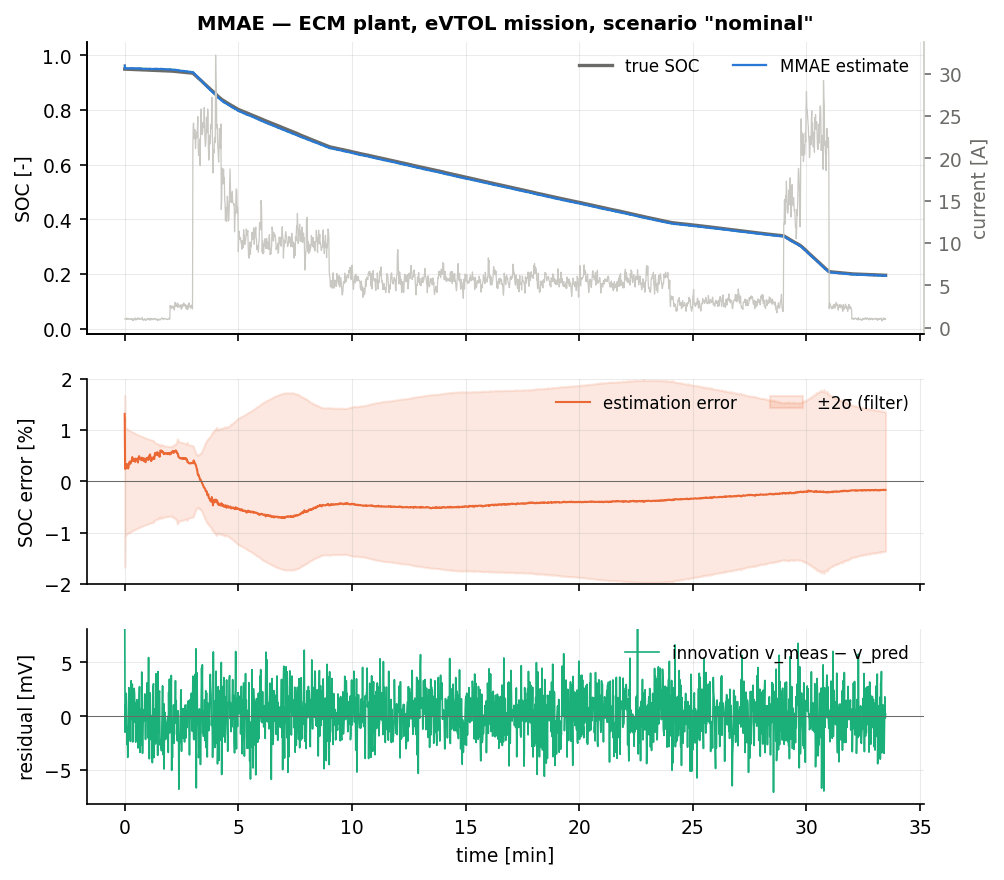
\includegraphics[width=\textwidth]{figures/cell_MMAE_nominal.png}
\caption{MMAE on the nominal eVTOL mission: true and estimated SOC (top), estimation error with the $\pm 2\sigma$ band when available (middle), voltage residual (bottom).}
\end{figure}
\begin{figure}[H]\centering
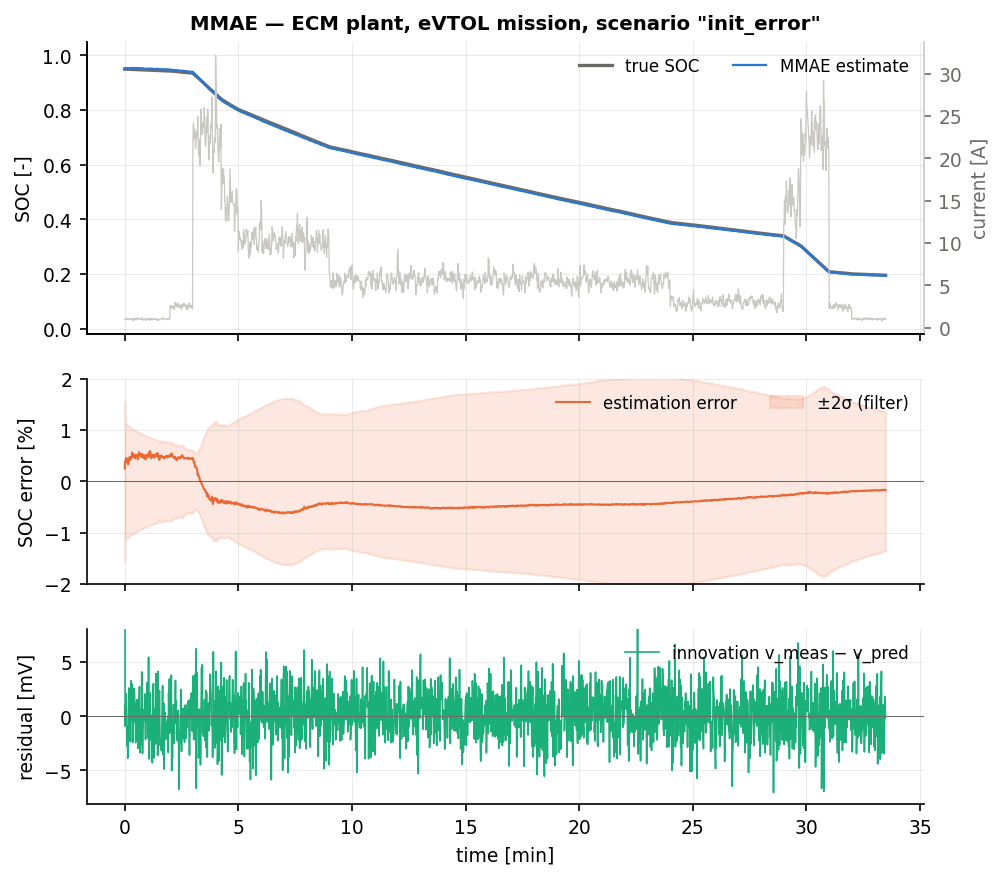
\includegraphics[width=\textwidth]{figures/cell_MMAE_init_error.png}
\caption{MMAE with a 35\,\% initial SOC error.}
\end{figure}
\begin{figure}[H]\centering
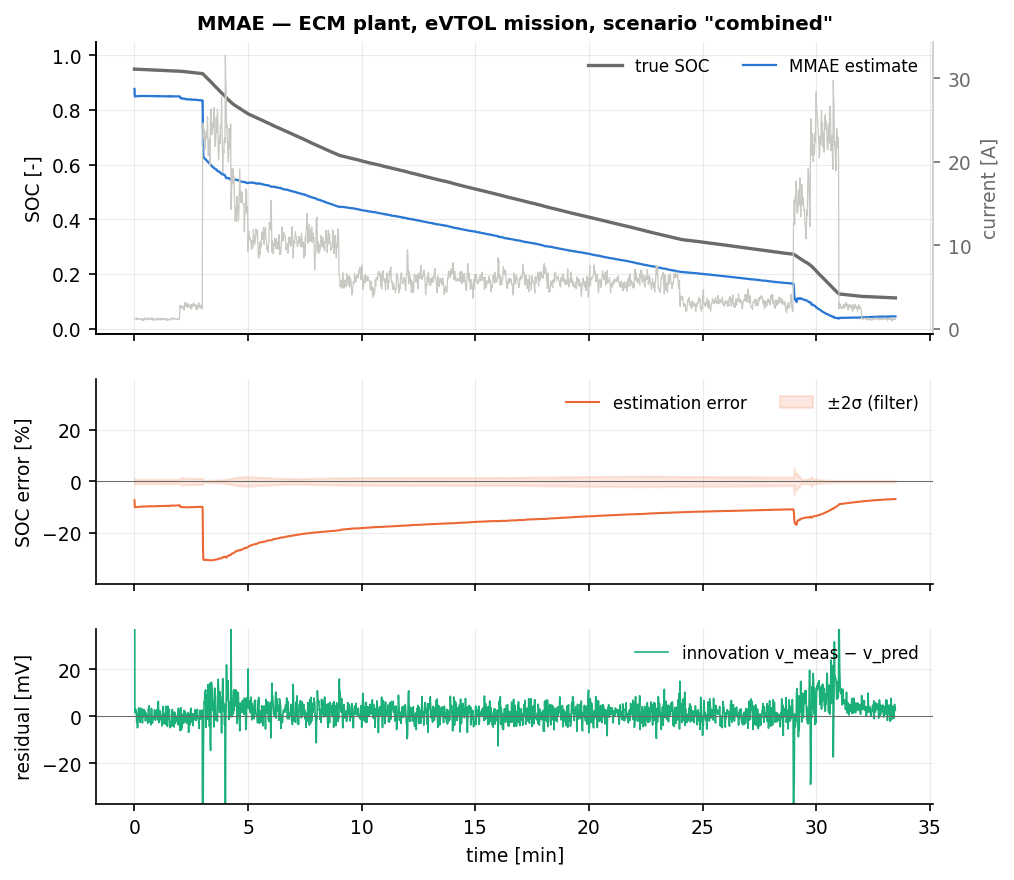
\includegraphics[width=\textwidth]{figures/cell_MMAE_combined.png}
\caption{MMAE on the \texttt{combined} scenario (25\,\% initial SOC error, \SI{150}{\milli\ampere} current bias, 2\,\% gain error, 10\,\% capacity loss with the associated resistance growth).}
\end{figure}
\begin{figure}[H]\centering
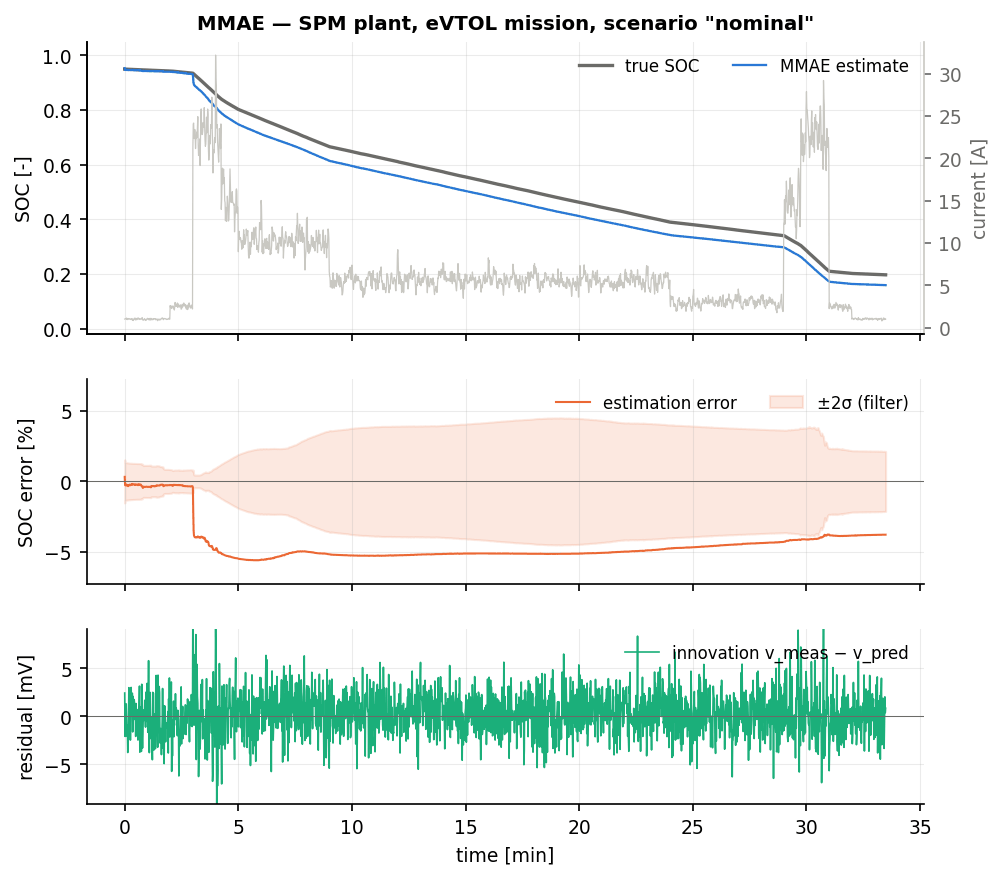
\includegraphics[width=\textwidth]{figures/cellspm_MMAE_nominal.png}
\caption{MMAE on the electrochemical (single-particle) plant, nominal mission: the estimator uses a 2-RC ECM fitted to that plant and therefore sees a structured \SI{4}{\milli\volt} residual instead of white noise.}
\end{figure}

All figures below are three-seed means in \% SOC, as tabulated above; the plain \texttt{EKF} run on
the same data is the reference (\texttt{EKF ref.} column).  For orientation, the EKF scores
$\mathrm{rmse}_{ss}$ = 0.05\,\% on \texttt{nominal}, 0.12\,\% on \texttt{noise\_step}, 0.21\,\% on
\texttt{outliers}, 0.46\,\% on \texttt{sensor\_dropout}, 1.36\,\% on \texttt{param\_mismatch},
1.52\,\% on \texttt{aged\_cell} and 12.44\,\% on \texttt{combined} (where it never converges), and
3.73\,\% on the nominal SPM mission.

\paragraph{Benign scenarios.}  \texttt{nominal}: $\mathrm{rmse}=0.42\,\%$,
$\mathrm{rmse}_{ss}=0.33\,\%$ against the EKF's $0.15\,\%$ / $0.05\,\%$, and the capacity estimate
settles at $\hat Q-Q=\SI{-0.001}{\ampere\hour}$, i.e.\ the bank reports a healthy cell to within one
gram of lithium.  The seven-fold SOC penalty relative to the EKF is the structural cost of the
mixture: the two wrong hypotheses each retain the floor weight $w_{\min}=0.01$ and each carries a
systematic SOC bias of $0.5$--$1.2\,\%$, and the inflated likelihood ($c_\mathrm{lik}=100$) makes the
posterior sharpen over roughly \SI{1900}{\second} rather than \SI{300}{\second}.  With
$c_\mathrm{lik}=1$ the nominal RMSE would be $0.26\,\%$; the extra accuracy is deliberately traded for
the noise robustness documented below.  Both values remain a factor of six inside the $2\,\%$
acceptance bound.  \texttt{init\_error} is statistically identical ($0.42\,\%$ / $0.36\,\%$,
$\hat Q-Q=\SI{-0.003}{\ampere\hour}$) and converges at $t=\SI{0}{\second}$.

\paragraph{Target scenario \texttt{aged\_cell}.}  The truth plant starts the mission with $15\,\%$
capacity loss, $Q^\star\approx\SI{4.25}{\ampere\hour}$, and the estimator is given the
beginning-of-life model.  The posterior moves off the nominal hypothesis within \SI{200}{\second} and
settles with most of its mass on $Q^{(2)}=\SI{4.5}{\ampere\hour}$; averaged over the last $10\,\%$ of
the mission the reported capacity error is $\mathbf{+\SI{0.410}{\ampere\hour}}$ against the
$+\SI{0.75}{\ampere\hour}$ that a non-SOH filter carries by construction.  The a-priori capacity error
is therefore cut by a factor of $1.8$, and the bank correctly identifies that the cell has aged.  It
does \emph{not} reach the true \SI{4.25}{\ampere\hour}, and by \eqref{eq:mm:logw} it cannot: the exact
Bayesian posterior concentrates on the nearest grid point, so the residual
$\SI{0.41}{\ampere\hour}$ is grid quantisation plus the softening effect of $c_\mathrm{lik}$, not an
estimation error.  A five-point bank at $\{100,95,90,85,80\}\,\%$ was evaluated in the development
sweep and does no better, because the finer grid also makes the hypotheses harder to distinguish under
the inflated likelihood.  The honest conclusion is that a bank resolves capacity to about half its
grid spacing; for finer SOH the joint or dual EKF of \cite{plett2004ekf3}, or a total-least-squares
capacity estimator \cite{plett2011awtls}, is the right instrument.  The SOC metrics on this scenario
are $\mathrm{rmse}=2.10\,\%$, $\mathrm{rmse}_{ss}=2.12\,\%$, worse than the EKF's $1.18\,\%$ /
$1.52\,\%$: the filter with the "right" capacity is not the filter with the best SOC here, because the
aged cell also has a $37.5\,\%$ larger $R_0$ that no hypothesis in the bank can represent, and the
mixture weights wander between hypotheses as the operating point moves along the OCV curve.

\paragraph{Robustness of the SOH estimate.}  The capacity error at the end of the mission is
$\SI{-0.001}{\ampere\hour}$ on \texttt{nominal}, $\SI{-0.003}{\ampere\hour}$ on \texttt{init\_error},
$\SI{+0.001}{\ampere\hour}$ on \texttt{current\_bias}, \texttt{sensor\_dropout} and
\texttt{preisach}, $\SI{-0.005}{\ampere\hour}$ on \texttt{noise\_step},
$\SI{-0.006}{\ampere\hour}$ on \texttt{outliers}, $\SI{-0.011}{\ampere\hour}$ on
\texttt{param\_mismatch}, $\SI{+0.018}{\ampere\hour}$ on \texttt{hot} and
$\SI{-0.064}{\ampere\hour}$ on \texttt{cold}.  In other words the bank does not falsely declare
capacity fade when the disturbance is a noisy sensor, an outlier-contaminated channel, a stuck
reading, a current-sensor bias, a wrong RC parameter set or a hysteresis model error --- a
false-positive rate below $0.25\,\%$ of the nominal \SI{5}{\ampere\hour} on eight of the ten
no-fade scenarios, $0.36\,\%$ on \texttt{hot} and $1.3\,\%$ on \texttt{cold}.  This is entirely due to the likelihood inflation \eqref{eq:mm:clik}: with
$c_\mathrm{lik}=1$, \texttt{noise\_step} alone produced a $19\,\%$ false capacity-fade declaration in
the development sweep.

\paragraph{Failure mode: parameter mis-attribution.}  On \texttt{combined} (true capacity
\SI{4.50}{\ampere\hour}) the bank reports $\hat Q-Q=\SI{+0.489}{\ampere\hour}$ --- it misses the fade
entirely --- and the SOC metrics are no better than the EKF's ($16.13\,\%$ / $12.56\,\%$ against
$16.02\,\%$ / $12.44\,\%$; $t_\mathrm{conv}=$ -- for both).  The reason is diagnostic rather than
accidental: in \texttt{combined} the dominant model error is the $25\,\%$ resistance growth, a
\emph{voltage} offset of \SI{16}{\milli\volt}, and the capacity dimension of the hypothesis space
simply cannot represent it.  Confirming the diagnosis, an EKF given $R_0\times1.2$ and the nominal
capacity scored $3.4\,\%$ / $0.6\,\%$ on the same scenario in the development sweep, a $4.7\times$ /
$20\times$ improvement over the baseline.  The lesson is general and worth stating plainly:
\textbf{a multiple-model bank answers the question it was given, whether or not that is the question
the data are about.}  The fix here is to let the bank span $R_0$ as well as $Q$ --- the class supports
it through \texttt{opts.p\_index}, and a two-dimensional grid would need $r=9$ filters --- or to
combine MMAE with one of the covariance-inflating filters of \cref{ch:stf} and \cref{ch:fadingekf},
which handle a voltage bias without needing to name it.

\paragraph{Other scenarios.}  \texttt{outliers}: $\mathrm{rmse}=0.41\,\%$,
$\mathrm{rmse}_{ss}=0.20\,\%$ against the EKF's $0.52\,\%$ / $0.21\,\%$ --- a modest gain.  The
inflated likelihood protects the \emph{weights}, but the individual filters still use the nominal
$\mR$ and are therefore as exposed to spikes as the EKF.  \texttt{preisach} (Preisach hysteresis with
the corrected sign convention in the truth plant): $0.81\,\%$ / $0.27\,\%$ against $0.58\,\%$ /
$0.20\,\%$ --- a $35\,\%$ regression in steady state, although the bank does converge immediately
against the EKF's \SI{16}{\second} and does not misread the hysteresis voltage as capacity fade.
\texttt{sensor\_dropout} is clearly worse ($0.94\,\%$ / $0.58\,\%$ against $0.72\,\%$ / $0.46\,\%$),
as is \texttt{param\_mismatch} ($1.70\,\%$ / $1.66\,\%$ against $1.28\,\%$ / $1.36\,\%$): in both, the
un-modelled effect is common to all three hypotheses, so the bank buys nothing and pays the mixture
penalty.  \texttt{cold} is the worst relative result ($1.12\,\%$ / $1.23\,\%$ against $0.20\,\%$ /
$0.16\,\%$), and it is also the only scenario with a visible capacity bias
($\SI{-0.064}{\ampere\hour}$): at $T=\SI{-10}{\celsius}$ the coloured innovations produced by the
slowed RC dynamics are read as weak evidence against the nominal hypothesis.  \texttt{hot}
($0.25\,\%$ / $0.13\,\%$ against $0.20\,\%$ / $0.03\,\%$) shows the mixture penalty in its purest
form: with no fault to detect, the floored weights on the two wrong-capacity hypotheses are the
entire error budget.

\paragraph{Cost.}  \SI{1752}{\nano\second}/step, $3.7\times$ the EKF's \SI{478}{\nano\second}, and
12.7\,kB of state in the straightforward implementation.

\paragraph{Electrochemical (SPM) plant.}  The SPM rows are MMAE's weakest showing, and the only case
in this family where an estimator is worse than the EKF on \emph{every} scenario of a plant.  On the
nominal SPM mission it reaches $\mathrm{rmse}_{ss}=4.69\,\%$ against the EKF's $3.73\,\%$ --- a
$26\,\%$ regression --- and the pattern repeats throughout (\texttt{cold} $8.75\,\%$ against
$7.35\,\%$, \texttt{sensor\_dropout} $6.35\,\%$ against $5.31\,\%$, \texttt{param\_mismatch}
$4.89\,\%$ against $3.13\,\%$, \texttt{init\_error} $4.83\,\%$ against $3.81\,\%$ and never reaching
the $2\,\%$ band).  Two effects compound.  First, the structured \SI{4}{\milli\volt} residual left by
the 2-RC ECM is common to all three hypotheses and cannot be explained by any of them, so the
posterior is driven by whichever filter happens to absorb it best rather than by capacity evidence;
the reported capacity errors, $\SI{-0.017}{\ampere\hour}$ to $\SI{-0.075}{\ampere\hour}$, are small
but systematically negative, i.e.\ the bank reads electrochemical model error as a slight capacity
fade.  Second, and more importantly, MMAE is the one filter in this chapter that adapts neither $\mR$
nor $\mP$: each member of the bank is a plain EKF with the nominal gain, so none of them shortens its
memory, and the mixture inherits the EKF's inability to stop the coulomb integrator from dominating
under structured model error --- and then adds the wrong-hypothesis bias of the floored weights on
top.  Where the $\mP$-inflating filters win by $5.7$--$10.4\times$ on this plant
(\cref{ch:fadingekf}, \cref{ch:stf}) and the $\mR$-adapting ones at least break even, a static
parameter bank has no mechanism at all for this class of error.  If SOH is needed on a cell whose
electrochemistry is not well captured by the estimator's ECM, the bank should be run \emph{on top of}
a covariance-inflating filter rather than on top of a plain EKF.

\section{Summary}
MMAE is the exact Bayesian answer to "which of these $r$ models generated the data", and for a
battery it is the cheapest way to get a state-of-health number out of an ordinary SOC filter: on a
cell with $15\,\%$ capacity loss it cuts the capacity error from \SI{+0.75}{\ampere\hour} to
\SI{+0.41}{\ampere\hour} and keeps the false-fade declaration below $0.25\,\%$ of capacity on eight
of the ten ECM scenarios where no fade is present (worst case $1.3\,\%$, on \texttt{cold}).  Use it when the unknown is a genuinely static parameter taking
a few plausible values and when a quantised answer is acceptable.  Always inflate the likelihood
covariance to budget for un-modelled error --- without it, a noisier voltage sensor alone makes this
filter declare $19\,\%$ capacity fade.  Always floor the weights and fold the floor back into the
recursion.  And do not expect the bank to explain an error that lies outside the parameter it
spans: on the combined-fault scenario it confidently reports a healthy cell because the actual fault
was in a dimension it was never given, and on the electrochemical plant --- where every member of the
bank inherits the plain EKF's gain and none of them shortens its memory --- it is the only estimator
in this family that is worse than the EKF on every scenario.  On a cell whose electrochemistry the
estimator's ECM does not capture, put the bank on top of a covariance-inflating filter, not on top of
a plain EKF.
